\chapter{Krav}\label{ch:krav}


Nu hvor der er lavet en god business model og case, vil kravene nu præciseres ud fra den systemvision der er lavet, og de use cases der er stillet op. Dette indgår i Elaboration fasen, som indeholder en bladning af at planlægge og modellere projektet. Dette betyder at de tidligere Use Cases implementeres, og det vil vise hvordan softwarens arkitektur beskrives og hvilke forudstæninger der bliver sat. Herunder befinder Krav, Analyse, Desing og Test aktiviterene sig under Elaboration fasen i Unified Process\cite{UnifiedProcess}. 

\section{Funktionelle krav}\label{sec:funktionelle-krav}
\section{Fully Dressed}

Herunder ses Fully Dressed Use Casen ‘Automatisk lagerstyring’. Use case 'Automatisk Lagerstyring' er bygget på de tidligere use cases: 'Afskriv vare', fordi den påvirker hvor meget der er på lager. 'Optælling af isbil', som er manuelt arbejde og vil nemt kunne erstattes med automatisk optælling. 'Bestil varer', dette ville gå hånd i hånd med automatisk optælling af bilen. Og til sidst use case 'Modtag varer', fordi systemet skal opdateres med de nye varer der kommer på lager. 

De alternative flows beskrevet i diagrammet er fundet gennem en diskussion, hvor mulige fejl eller forhindringer kan opstå under flowet af handlinger. De alternative flows beskriver, hvordan et system kan fejle undervejs, hvad der er nødvendigt at være forberedt på, og hvordan disse alternative flows kan behandles så systemet ikke stopper, men kan fortsætte Use Casen til ende. Sker det at systemet eller kunden ikke opfører sig som forventet, skal de mulige udfald udtænkes, og sådanne scenarier skal kunne behandles af systemet så vidt muligt.


\begin{longtable}{ |p{120pt}|p{120pt}|p{120pt}| }
    \hline
    \textbf{Use case navn} & Automatisk lagerstyring & \\
    \hline
    \textbf{Aktør} & Depotchefen & \\
    \hline
    \textbf{Præbetingelser} & Et lager med en addresse, penge til at bestille, lagerbeholding fysisk er det samme som i systemet, having a little bit sales data & \\
    \hline
    \textbf{Postbetingelser} & Et lager det er opfylgt med IS & \\
    \hline
    \textbf{Frekvens} & 1 gang om dagen & \\
    \hline
    \textbf{Main Success Scenario} (Flow of events) & \textbf{Aktørhandling} & \textbf{Systemsvar} \\
    \hline
    & 1. vis salgs statistik & 2. en hel masse statistik \\
    \hline
    & 3. klikker "generer lagerplan" & 4. fil dialog omkring hvor planen skal gemmes og er automaitsk sendt til plan-fanen \\
    \hline
    & 5. klikker "load plan" & 6. en eller anden form for UX feedback \\
    \hline
    \textbf{Alternative flows} & 5a. Aktøren vil gerne modificere planen, og gør det i plan-fanen \\
    \hline
\end{longtable}

\begin{longtable}{ |p{120pt}|p{120pt}|p{120pt}| }
    \hline
    \textbf{Use case navn} & Automatisk bogføring & \\
    \hline
    \textbf{Aktør} & Depotchefen & \\
    \hline
    \textbf{Præbetingelser} & ingen & \\
    \hline
    \textbf{Postbetingelser} & bogføring er automatisk færdiggjord i et excel ark & \\
    \hline
    \textbf{Frekvens} & 1 gang om dagen & \\
    \hline
    \textbf{Main Success Scenario} (Flow of events) & \textbf{Aktørhandling} & \textbf{Systemsvar} \\
    \hline
    & 1. klikker "export bogføring" & 2. systemet exporter en excel fil med bogføring \\
    \hline
\end{longtable}

\section{Informationskrav}\label{sec:informations-krav}
Informationskravene omhandler hvilke informationer systemet skal registrere, sådan at modeller 
kan designes, som binder konceptuelle klasser sammen.

\subsection{Domænemodel}\label{Domainmodel}
Domænemodellen \cite{Larman2004} beskriver de relationer klasserne har til hinanden, samt hvilke attributter de indeholder. Her laves Domænemodellen ud fra Kandidatklasserne og tilhørende arkitekturprincipper.

\begin{landscape}
\begin{figure}[p]
    \centering
    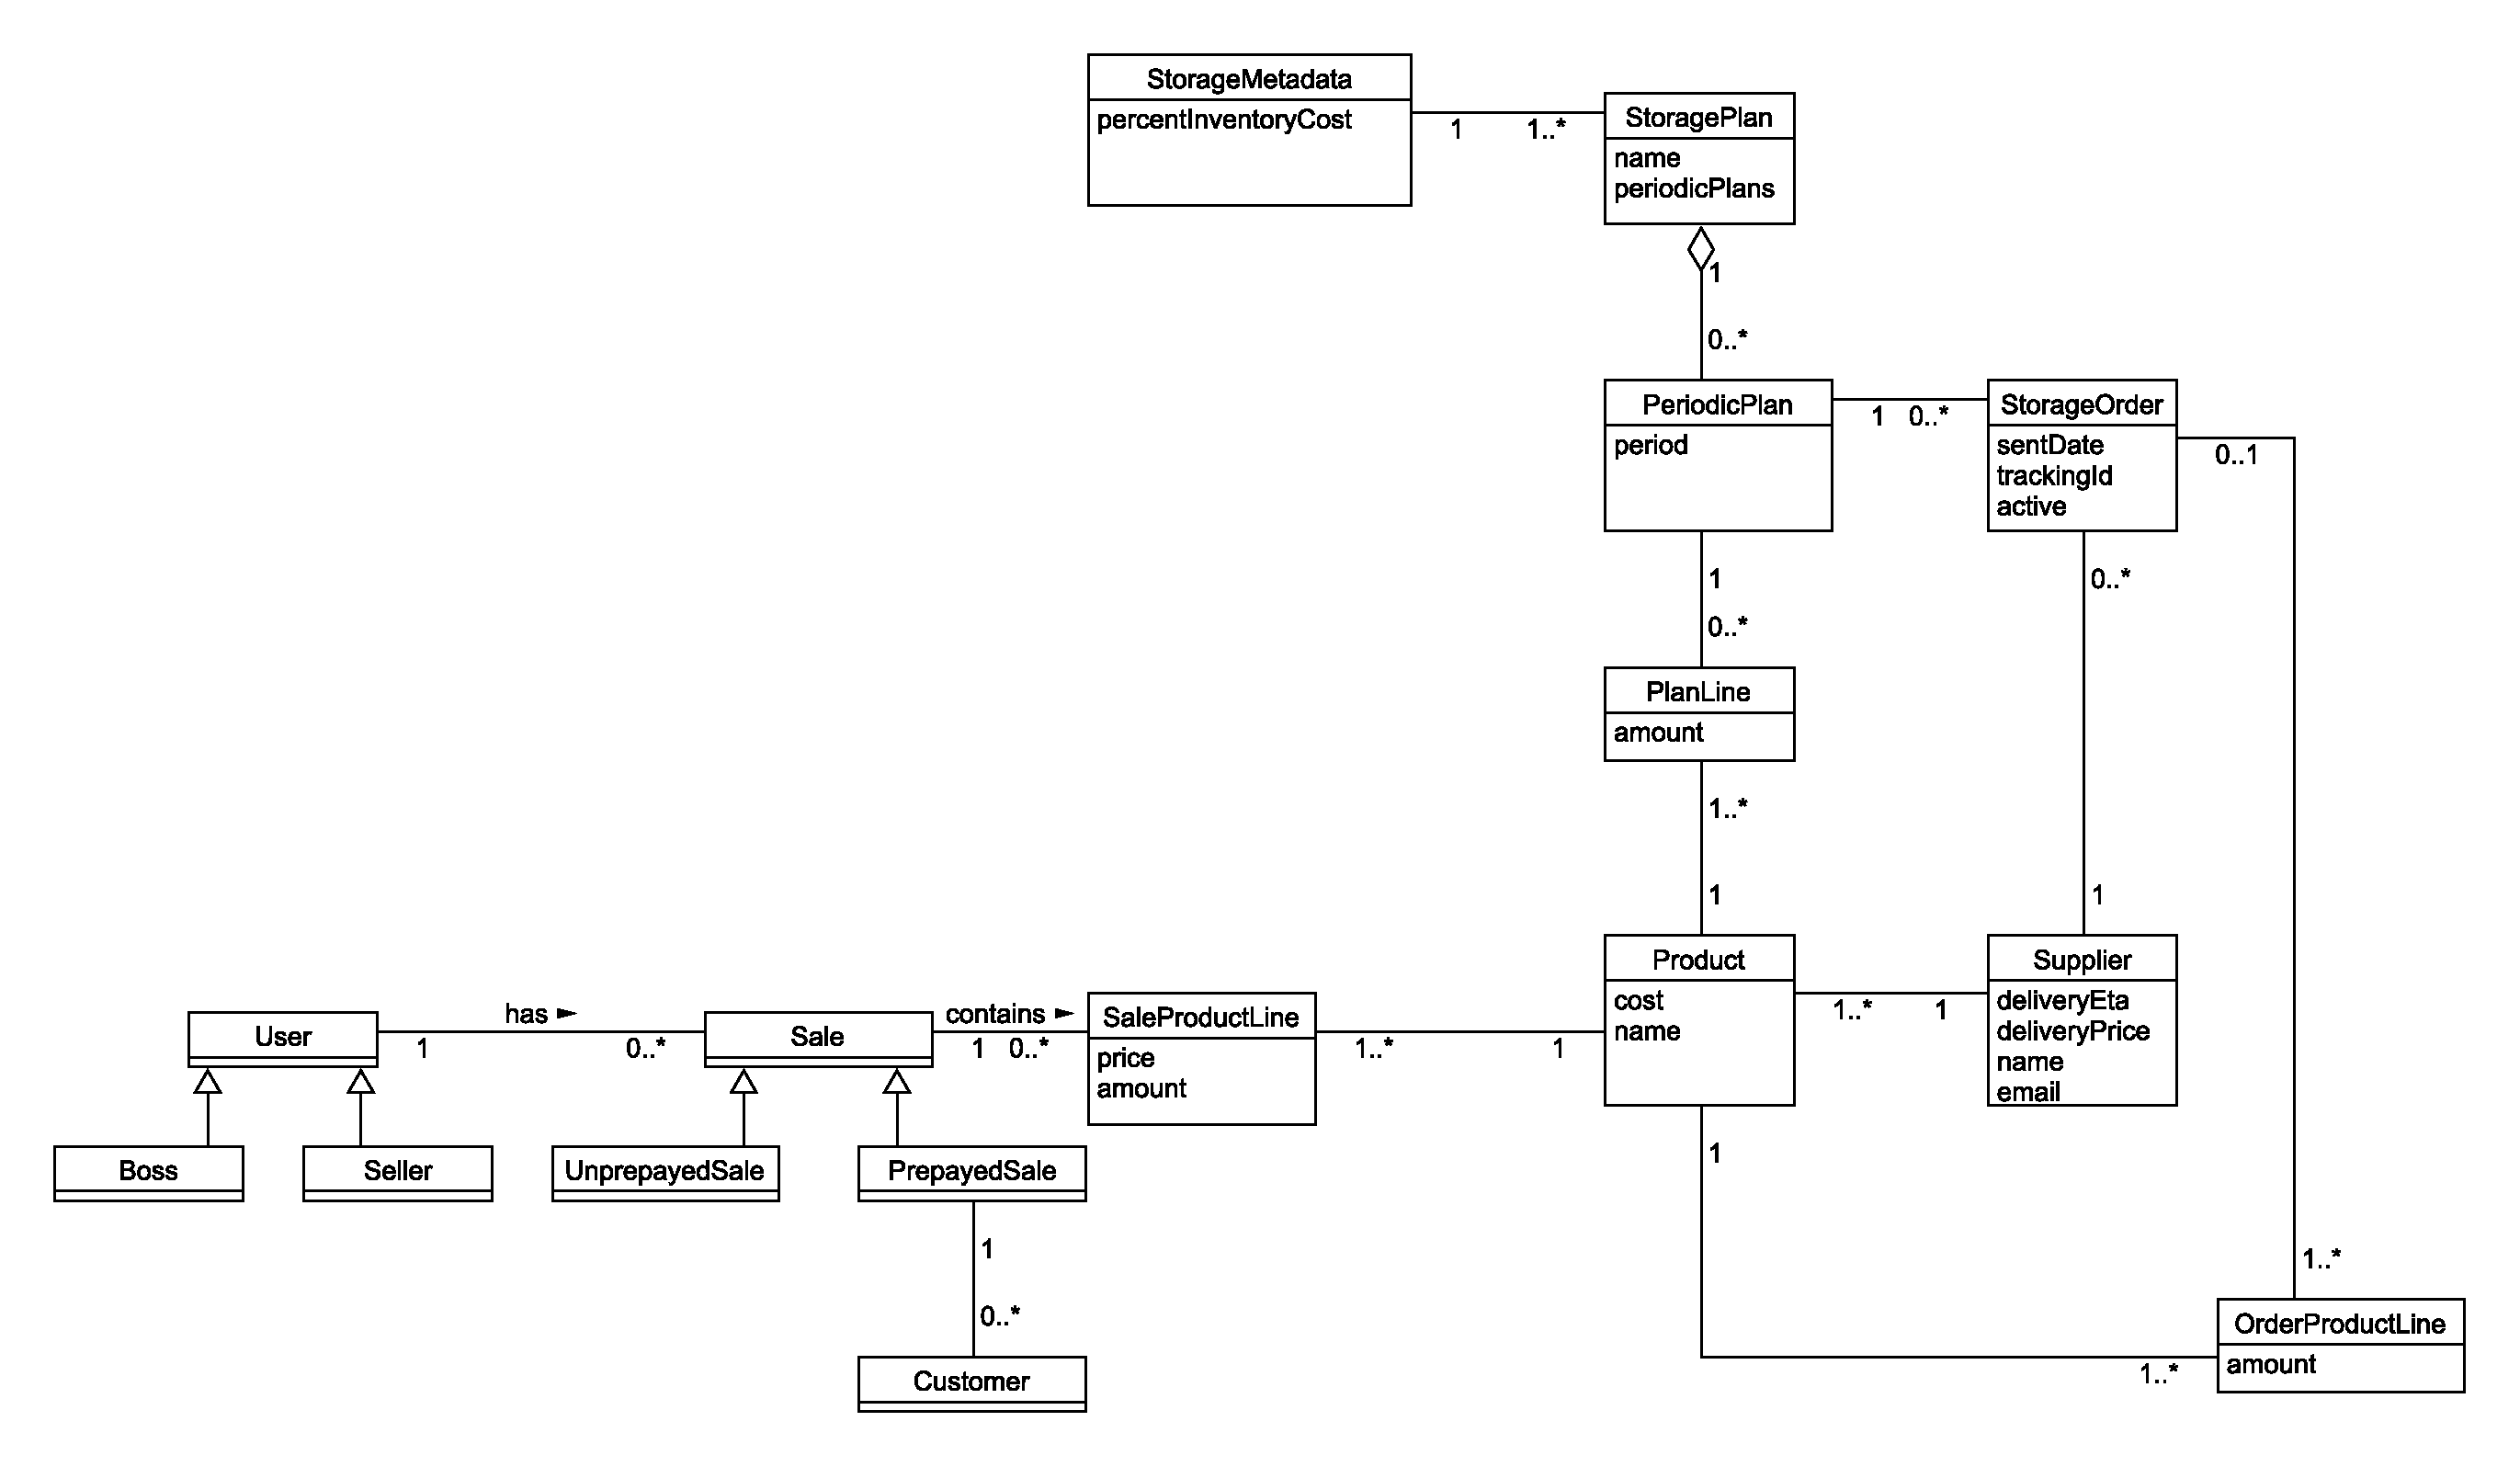
\includegraphics[width=0.9\hsize]{figures/krav/domain_model_1.eps}
    \caption{Domænemodel 1}
    \label{fig:domain_model}
\end{figure}
\end{landscape}

Domænemodellen som ses ovenfor på Figur \ref{fig:domain_model} viser, hvordan klasserne er repræsenteret og hvilke relationer de har til hinanden. SeasonalPlan er planen, som beskriver hvordan lageret skal være hos Hjem-IS. Sæsonplanen for lagerbeholdningen bestemmes af hvilke produkter der er på lager, og hvor meget der bliver solgt. Ud fra dette kan der laves en bestilling (StorageOrder), som indeholder informationer om, hvilke produkter der skal bestilles, hvor mange, og hvilken Supplier de skal bestilles fra. Disse bestillingsplaner bestemmer sæsonplanen.
For at kunne gennemføre Use Casen er det ikke nødvendigt endnu at tage højde for Sales og Users, da det kun er Products og Storage ændringer, der er relevante. 

\begin{figure}[H]
    \centering
    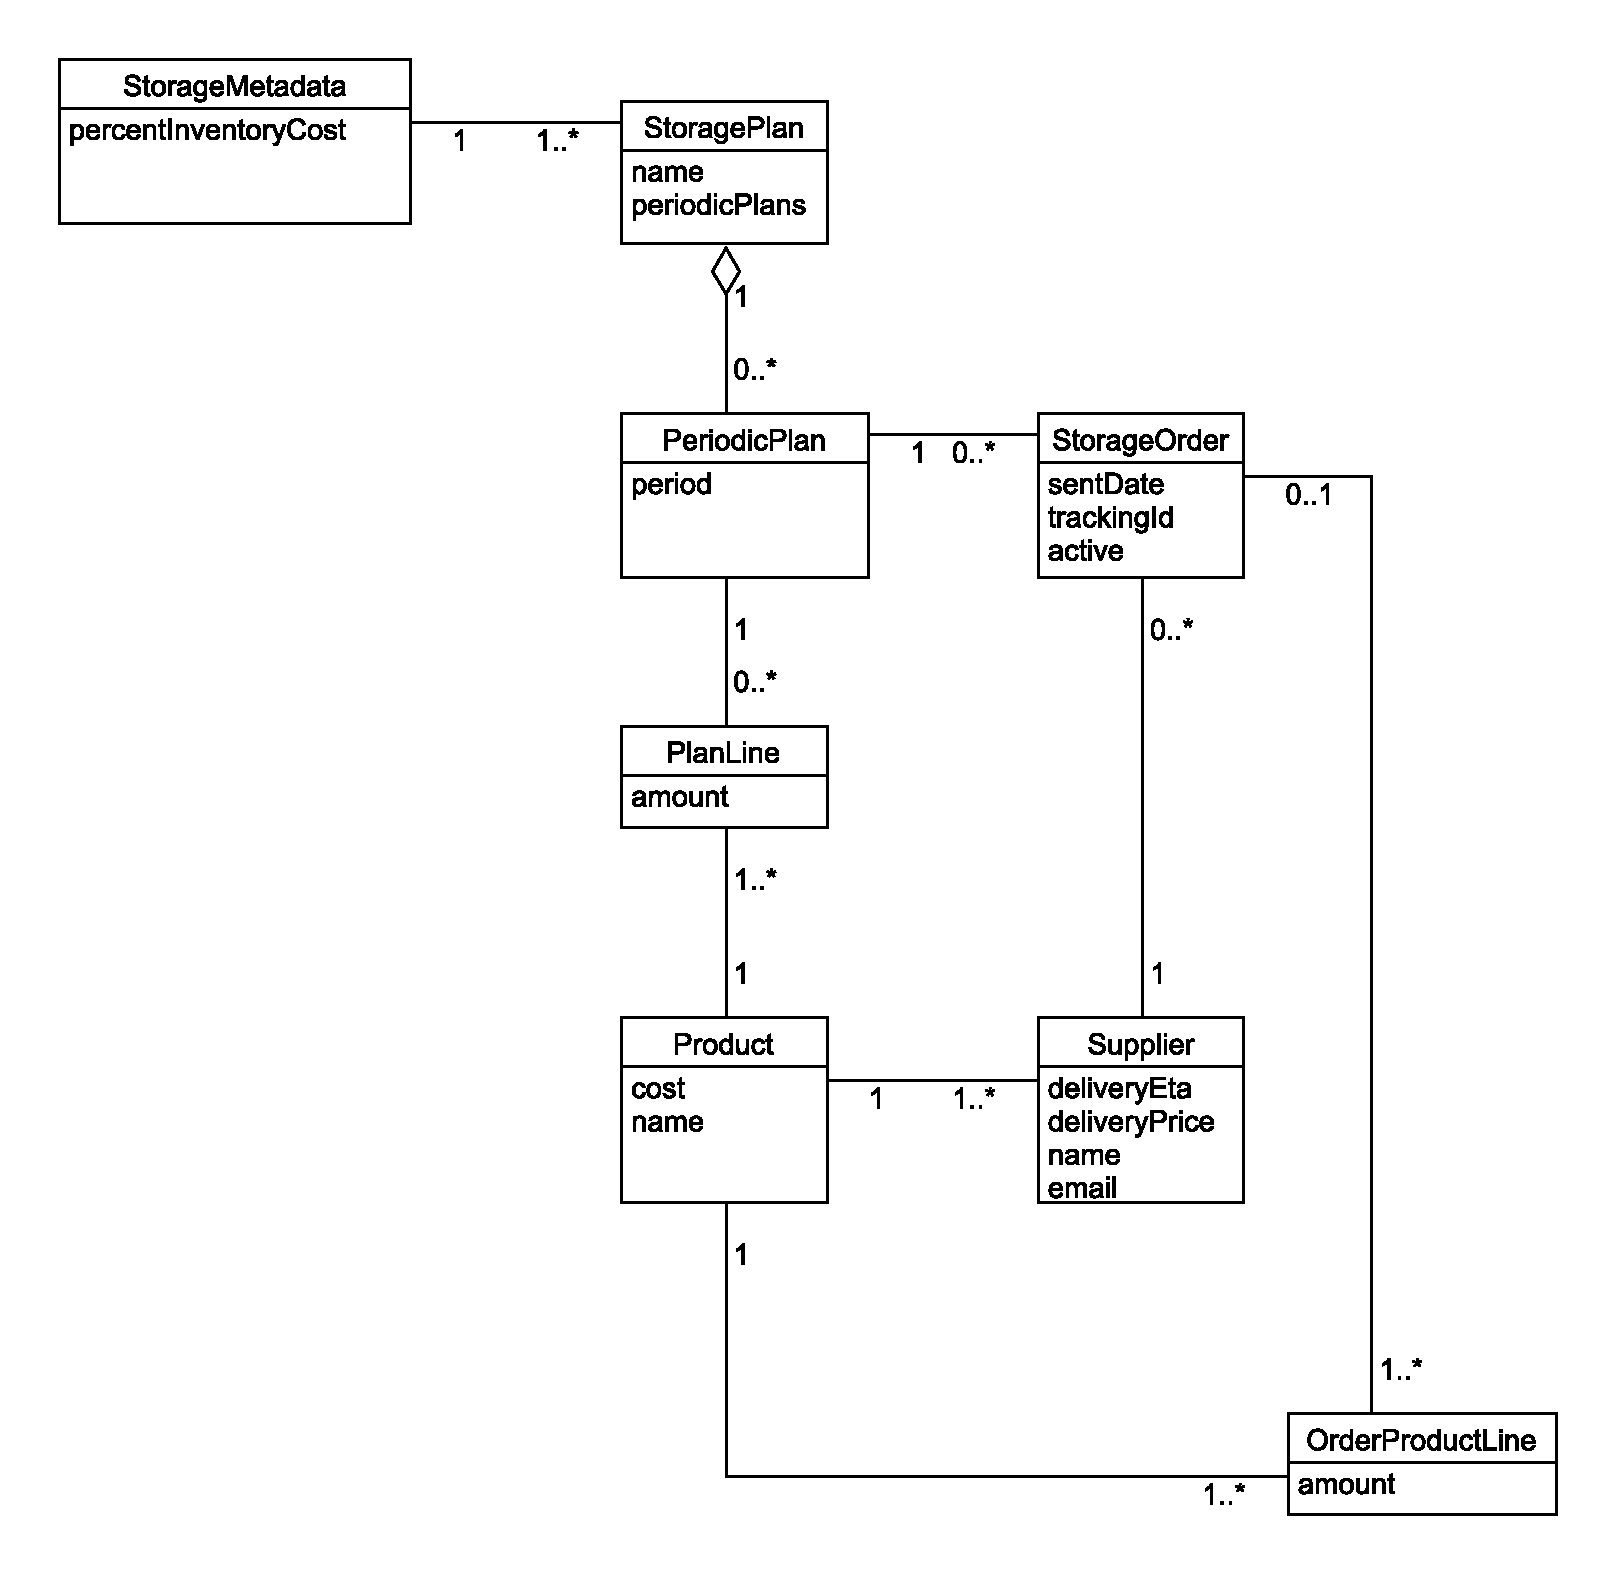
\includegraphics[width=0.9\textwidth]{figures/krav/domain_model_2.eps}
    \caption{Domænemodel 2}
    \label{fig:domain_model_2}
\end{figure}

Domænemodellen ovenfor forholder sig kun til de relevante klasser for at kunne gennemføre Use Casen Automatisk Lagerstyring. Det er ud fra denne at databasen vil blive designet.

\subsection{Relationelle modeller}
Domænemodellen er på plads og der kan udvikles en Relational model af databasen \cite{DatabaseSystems}. Der vil først tages udgangspunkt i at mappe hver klasse til en tabel, hvor der tages højde for klassenavn og attributter.
Da der ingen nedarvning er mellem nogen af klasserne, er det ikke relevant at tænke i pull-up og pull-down \cite{Larman2004}. Hver klasse får derfor sin egen tabel.
Dernæst skal associationerne laves ud fra, om der er tale om 1-til-1, 1-til-mange eller mange-til-mange relationer \cite{DatabaseSystems}. 

\begin{figure}[H]
    \centering
    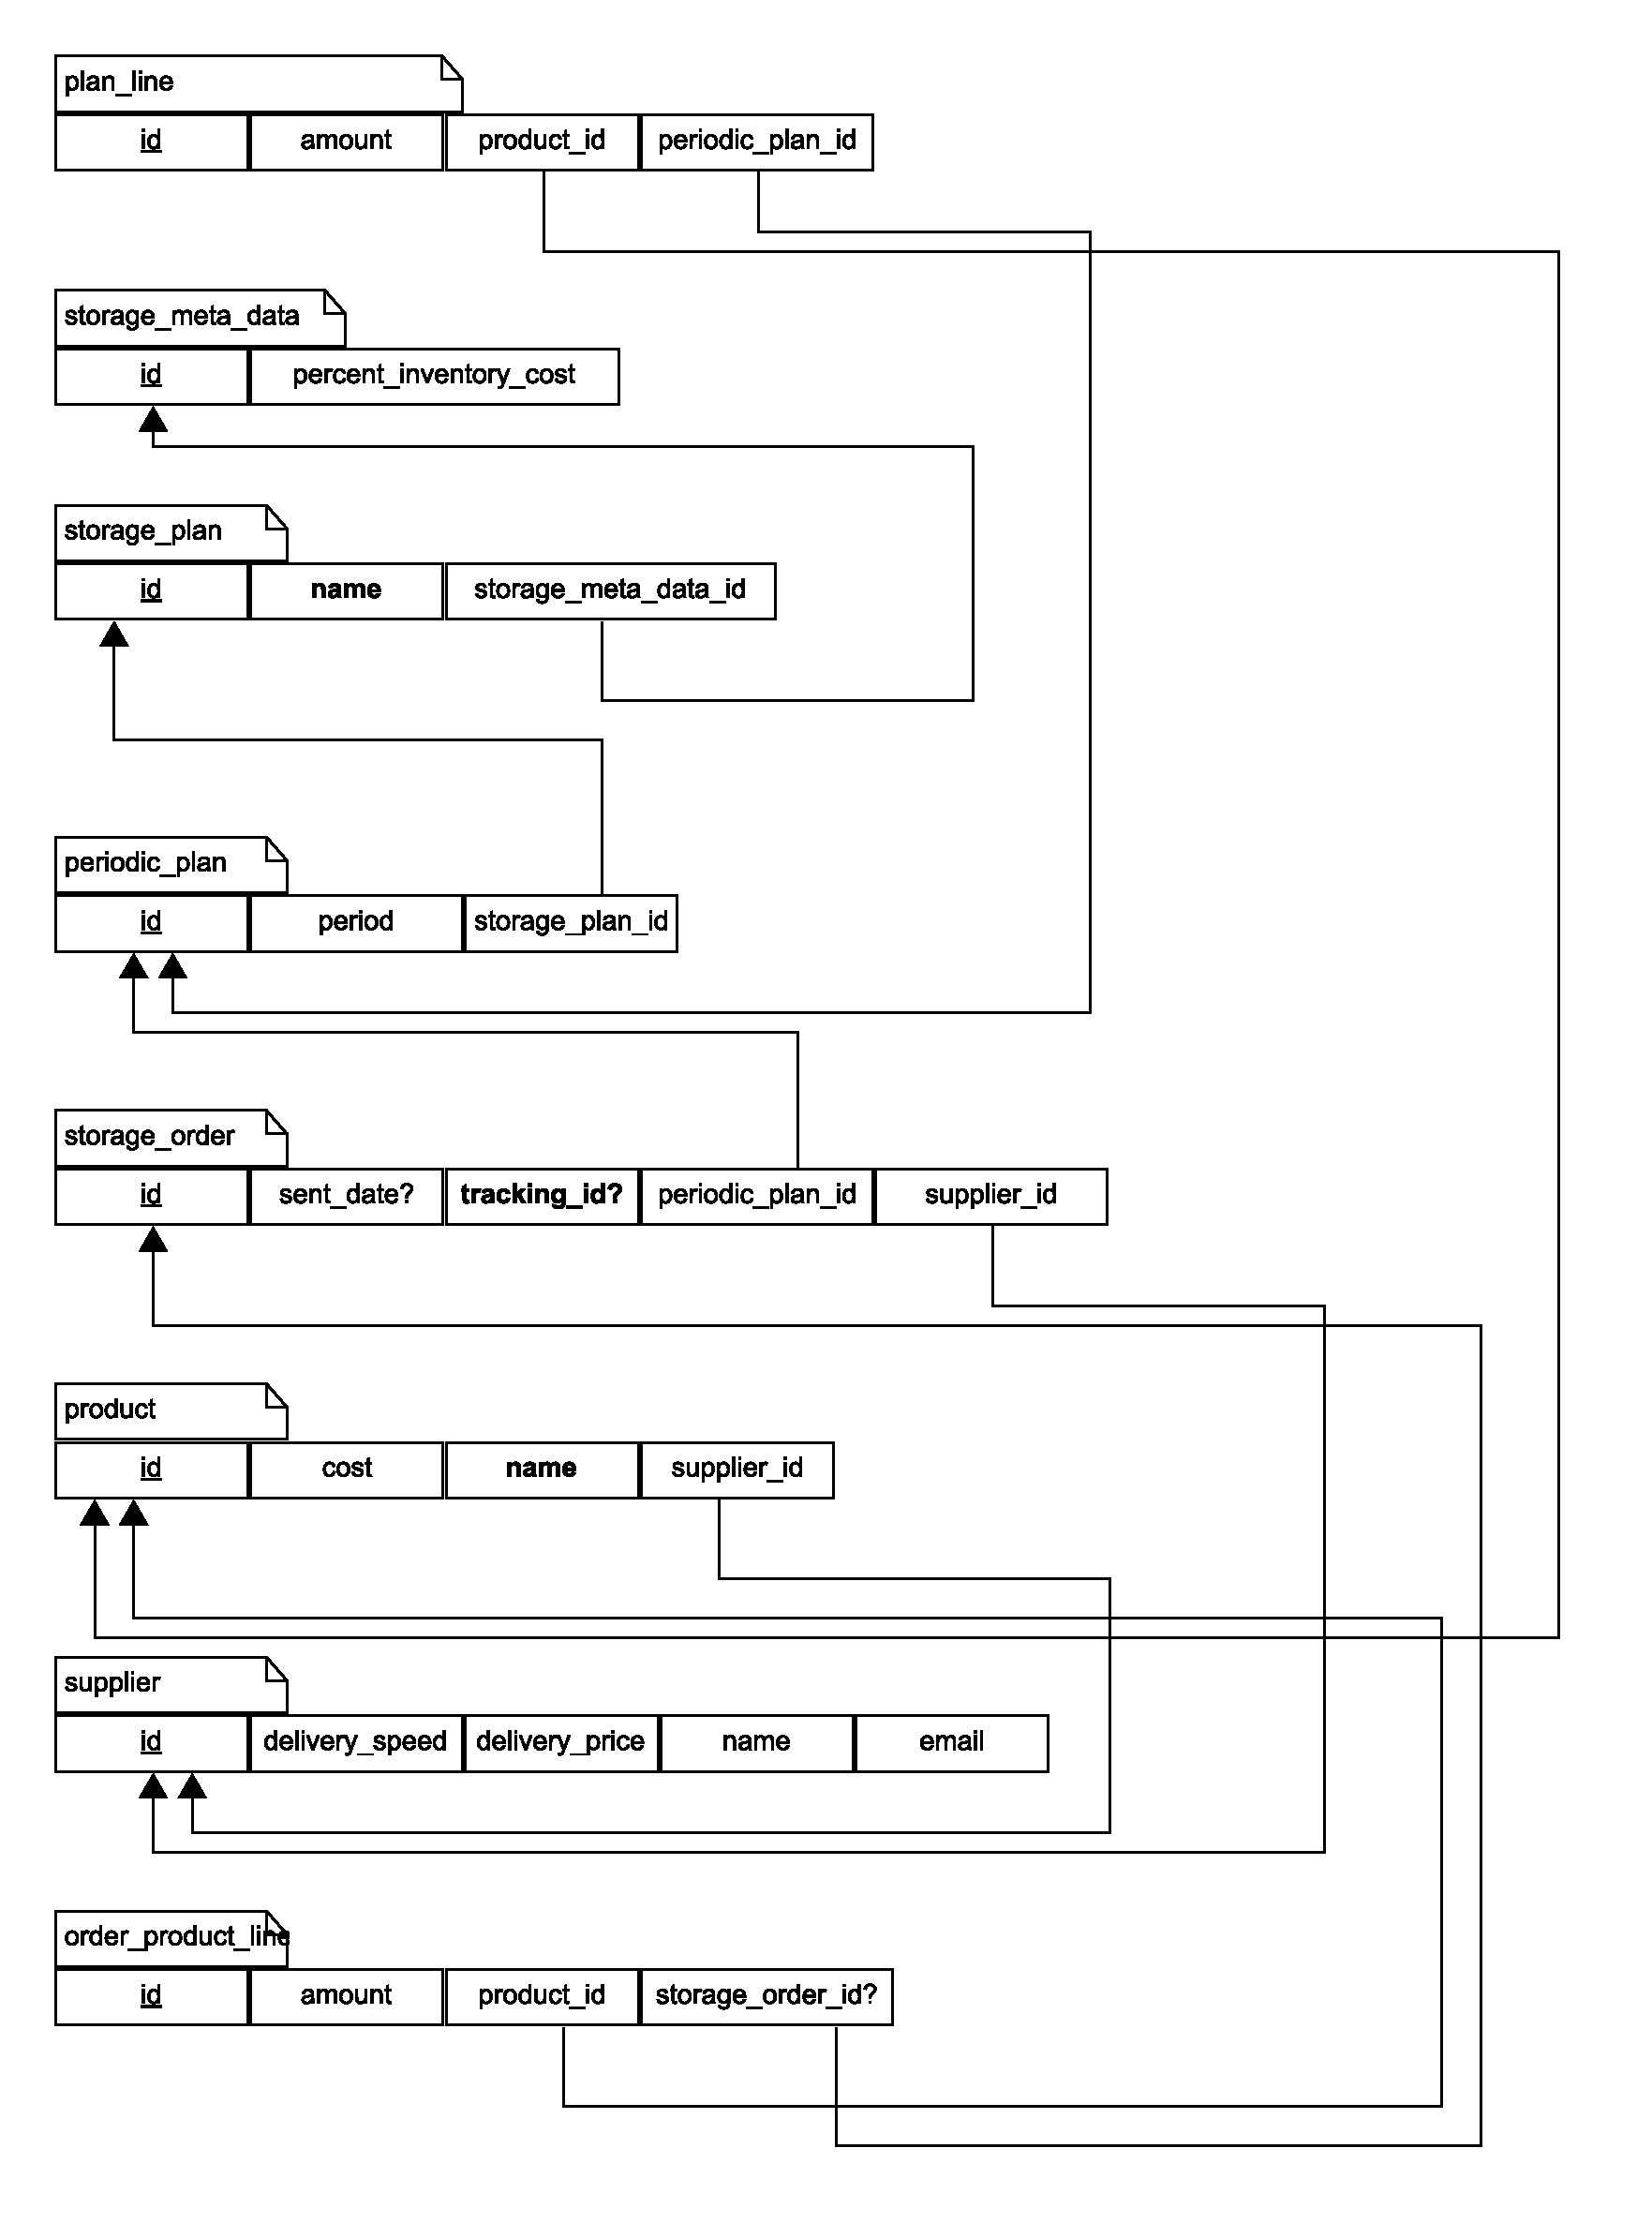
\includegraphics[width=0.9\textwidth]{figures/krav/relation_model_0th_normalization.eps}
    \caption{Relationsmodel før normalisering}
    \label{fig:relational_model_0}
\end{figure}

Reglerne for de forskellige relationer og hvordan de skal forbindes er fulgt under udviklingen af den Relationelle model, hvilket bl.a. kan ses på 'product\_supplier' tabellen. Denne forbinder en mange-til-mange association mellem Product og Supplier. 
Nu hvor tabellen er lavet, kan den normaliseres. Der vil blive normaliseret ud fra 4 normalformer: 1NF, 2NF, 3NF og Boyce-Codd Normalform (BCNF) \cite{DatabaseSystems}.

Efter at have kigget tabellen igennem kan det ses, at 1NF er opfyldt da alle værdier er atomiske.
For at opfylde 2NF skal 1NF være opfyldt, og der skal ikke være nogle partial dependencies. Da der skal bruges en Map mellem 'products' og 'seasonal\_plans' laves der en ny tabel: 'seasonal\_plan\_product\_maps'. Denne vil også indeholde 'amount'.

\begin{figure}[H]
    \centering
    \includegraphics[width=0.9\textwidth]{figures/krav/relation_model_1th_normalization.eps}
    \caption{Relationsmodel efter 2NF}
    \label{fig:relational_model_1}
\end{figure}

For at opfylde 3NF skal 2NF være opfyldt, og der må ikke være nogle transitive afhængigheder \cite{DatabaseSystems}. Det minder meget om kravet til 2NF, og det kan konkluderes at der ingen transitive afhængigheder er.
For at opfylde BCNF kræves det at 3NF er opfyldt og at samtlige determinanter er kandidatnøgler. De determinanter, der er I den relationelle model er samtlige attributter med 'id' og '...\_id' på nær 'tracking\_id'. 'tracking\_id' og 'sent\_date' kan være null når tuplen oprettes, og opdateres senere. Der er derfor kun kandidatnøgler.
Det kan nu konkluderes at den relationelle model er på BCNF og kan udvikles i Microsoft SQL med Microsoft SQL Server Management Studio \cite{MSSQL}. Først skal der laves en analyse over systemet ud fra de funktionelle krav og informationskrav der er stillet op indtil videre. 

 